\documentclass[11pt]{article}

% parameters are fairly self-explanatory here, thankfully
\usepackage[width=7in,height=9.5in,top=0.75in,centering]{geometry}

% for math-ing
\usepackage{amsmath}
\usepackage{amssymb}


%%%%%% tables %%%%%%%%

\usepackage{array}
\renewcommand{\arraystretch}{1.5}
\setlength{\tabcolsep}{8pt}

%%%%%% plotting %%%%%%

\usepackage[dvipsnames]{xcolor}
\usepackage{tikz}
\usepackage{pgfplots}

\pgfplotsset{every axis/.append style={
                    axis x line=middle,    % put the x axis in the middle
                    axis y line=middle,    % put the y axis in the middle
                    axis line style={<->,color=black}, % arrows on the axis
                    xlabel={$x$},          % default put x on x-axis
                    ylabel={$y$},          % default put y on y-axis
            }}
            
 \pgfplotsset{compat=1.14} % sometimes, everything falls apart without this
 
 %\usepgfplotslibrary{fillbetween} %for shading between curves

%%%%%% commands %%%%%%

% exam heading; course name is first argument, exam information is second argument
\newcommand{\Heading}[2]{
    \fbox{
        {\Large\textbf{#1}}
        }
    \hfill
    \fbox{
        \begin{minipage}{0.2\textwidth}
            \begin{center}
            \textbf{#2}
            \end{center}
        \end{minipage}
    }
    \par\vspace{0.1in}}

% for being lazy while beautifying integrals
\newcommand{\dint}{\displaystyle\int}

% for being lazy while beautifying limits
\newcommand{\dlim}{\displaystyle\lim}

%%%%%% stuff %%%%%%

\usepackage{fancyhdr}

%\setcounter{page}{0} % first page is page 0

\parindent0pt % no indent

\fboxsep=0.25cm % little space in fbox border

%%%%%% BEGIN! %%%%%%%

\begin{document}

\pagestyle{fancy}

% record goals here to create sense of transparency

\fancyhead[c]{%
  \ifcase\value{page}
  % empty test for page = 0
  \or
  \or {\bf\color{ForestGreen} FE1(D1): Meaning of a Derivative}% page=1
  \or {\bf\color{ForestGreen} FE2(D3): Derivatives of Basic Functions}% page = 2
  \or {\bf\color{ForestGreen} FE3(D2): Compute Derivatives}% page = 3
  \or {\bf\color{Fuchsia} FE4(I1): Meaning of an Integral}% page = 4
  \or {\bf\color{Fuchsia} FE5(I3): Antiderivatives and Indefinite Integrals}% page = 5
  \or {\bf\color{Fuchsia} FE6(I4): Compute Definite Integrals}% page = 6
  \or {\bf\color{ProcessBlue} FE7(F3): Summations}% page = 7
  \or {\bf\color{RoyalBlue} FE8(L1): Limits and Continuity}% page = 8
  \or {\bf\color{Orange} FE9(P1): Discrete Random Variables}
  \or {\bf\color{Orange} FE10(P2): Continuous Random Variables}
  \else
  % Empty chead here!
  \fi
}

\thispagestyle{empty} % don't display that this is page 0

\Heading{MATH 1190/1210 Survey of Calculus I}{Final Exam\\Growth-Based\\Fall 2025\\Part 1}

\vspace{0.1in}

\textbf{Name} \hrulefill \, \begin{minipage}{0.16\textwidth}\begin{center}\textbf{UVA ID\\ (e.g. hdj4nd)} \end{center}\end{minipage}\hrulefill\\

\begin{minipage}{0.2\textwidth}\begin{center}\textbf{Course \&\\ Section Number} \end{center}\end{minipage} \hrulefill\,\,\textbf{Date} \hrulefill  \\

\hrulefill
\paragraph*{Course \& Section Numbers:}

{\small
\begin{center}
\begin{tabular}{| c | c | c | c | c |}
\hline
%
\begin{minipage}{0.12\textwidth}\begin{center}
1190-100\\
J. Rolf\\
(11:00 AM)
\end{center}\end{minipage}
&
\begin{minipage}{0.12\textwidth}\begin{center}
1190-200\\
J. Rolf\\
(9:30 AM)
\end{center}\end{minipage}
&
\begin{minipage}{0.12\textwidth}\begin{center}
1210-100\\
Mikhail\\
(8 AM)
\end{center}\end{minipage}
&
\begin{minipage}{0.12\textwidth}\begin{center}
1210-200\\
Raul\\
(9:30 AM)
\end{center}\end{minipage}
&
\begin{minipage}{0.12\textwidth}\begin{center}
1210-300\\
Sherman\\
(11 AM)
\end{center}\end{minipage}
\\
%
\hline
%
\begin{minipage}{0.12\textwidth}\begin{center}
1210-400\\
Sherman\\
(12:30 PM)
\end{center}\end{minipage}
&
\begin{minipage}{0.12\textwidth}\begin{center}
1210-500\\
Michael\\
(2 PM)
\end{center}\end{minipage}
&
\begin{minipage}{0.12\textwidth}\begin{center}
1210-600\\
J. Bowling\\
(3:30 PM)
\end{center}\end{minipage}
&
\begin{minipage}{0.12\textwidth}\begin{center}
1210-700\\
Josh\\
(9:30 AM)
\end{center}\end{minipage}
&
\begin{minipage}{0.12\textwidth}\begin{center}
1210-800\\
Mason\\
(2 PM)
\end{center}\end{minipage}
\\
%
\hline
%
\begin{minipage}{0.12\textwidth}\begin{center}
1210-900\\
Caelan\\
(3:30 PM)
\end{center}\end{minipage}
&
\begin{minipage}{0.12\textwidth}\begin{center}
1210-920\\
Caelan\\
(5 PM)
\end{center}\end{minipage}
&
\begin{minipage}{0.12\textwidth}\begin{center}
1210-940\\
Mitchell\\
(10 AM)
\end{center}\end{minipage}
&
\begin{minipage}{0.12\textwidth}\begin{center}
1210-950\\
Mitchell\\
(11 AM)
\end{center}\end{minipage}
&
\begin{minipage}{0.12\textwidth}\begin{center}
1210-960\\
Mitchell\\
(noon)
\end{center}\end{minipage}
\\
\hline
\end{tabular}
\end{center}

}

{\small

\paragraph*{Instructions:}

\begin{itemize}
    
    \item The regular time allowed for completing this assessment is \fbox{$100$} minutes.
    %\item This assessment is out of 50 points.\\ 
    \item This assessment contains one single-part or multi-part problem for each of the following targets: \textbf{FE1(D1), FE2(D2), FE3(D3), FE4(I1), FE5(I3), FE6(I4), FE7(F3), FE8(L1), FE9(P1), FE10(P2)}.
    \item On each problem, you will receive a score of Exceeds Expectations (5), Proficient (4), Almost (3), Developing (2), Emerging (1), or Not Yet (0). %{\bf Please do not interpret your score as a percentage.}
    \item \textbf{It is to your best interest to complete all problems on this exam and not leave anything black.} The Final Exam learning targets count separately. If a problem is skipped, you will earn a Not Yet (0) on the corresponding Final Exam learning target, which could impact your final negatively and significantly.
    \item Your performance on each of the Final Exam targets can replace your scores on corresponding targets from Knowledge Checkpoints given during the semester, if your performance on the Final Exam is higher.
    %\item You will have opportunities to reassess on the targets appearing on this assessment after the next {\bf 2} assessments.\\
    \item You may NOT use calculators, dictionaries, notes, phones, or any other kind of aid.
    \item Please write neatly. What cannot be read, cannot be graded.
    \item Carefully work out each problem and clearly indicate your final answer to every problem.
    \item Throughout, give the most descriptive answer possible. \textbf{For instance, ``DNE" will not be accepted when ``$=\infty$" is applicable.}
    %\item Please provide the most specific answer possible. For instance, if a limit does not exist because it goes to $\infty$ or $-\infty$, then specify this.
    \item Please use the methods discussed up to this point in the course. For example, any work based on l'H\^opital's Rule will not receive credit.
    \item \textbf{All work must be shown unless otherwise specified.} Partial credit will not be given if appropriate work is not shown.
    \item In particular, {\bf any answer appearing with no justification will receive no credit regardless of whether the answer was correct}, unless otherwise specified.
    \item Please first respond to the prompts on which you feel most proficient, then respond to others later.
    \item This booklet is printed double-sided. It contains 14 pages and 10 numbered problems.
    \end{itemize}
    
    }

\vfill


%%%%%%%%%

\newpage%
%%%%%%%%%


\begin{enumerate}

%%%%%%%%%%%%%%%%%%%%%%%%%%%%%%%%%%%%%%%%%%%%%%%%%%%%%
%%%%%%%%%%% BEGIN PROBLEM D1 %%%%%%%%%%%%%%%%%%%%%%%%
%%%%%%%%%%%%%%%%%%%%%%%%%%%%%%%%%%%%%%%%%%%%%%%%%%%%%

\item Sketch an example of a function $f$ such that $f'(1)$ does not exist, but $f$ is continous at $1$.
    
    \begin{center}
        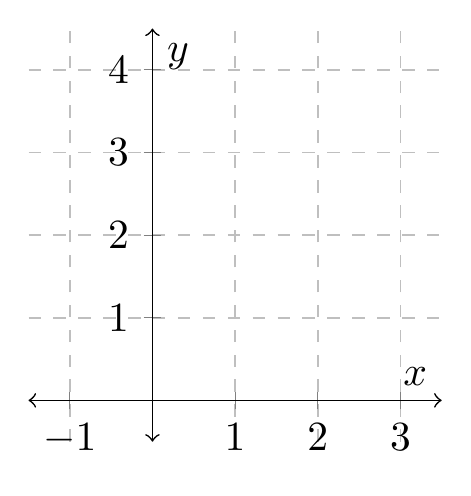
\begin{tikzpicture}[scale=1.5]
              \begin{axis}[
            %    axis y line = left,
            %    axis x line = bottom,
                xlabel={$x$},
                xtick       = {-1,1,2,3,4},
                xticklabels = {$-1$,1,2,3,4},
                ytick       = {1,2,3,4},
                yticklabels = {1,2,3,4},
                samples     = 160,
                domain      = -1:5,
                restrict y to domain=-1:5,
                xmin = -1.5, xmax = 3.5,
                ymin = -0.5, ymax = 4.5,
                grid=both, grid style=dashed,
                width=2in, height=2in
              ]
            \end{axis}
        \end{tikzpicture}
        \end{center}


%%%%%%%%%%%%%%%%%%%%%%%%%%%%%%%%%%%%%%%%%%%%%%%%%%%%%
%%%%%%%%%%% END PROBLEM D1 %%%%%%%%%%%%%%%%%%%%%%%%%%
%%%%%%%%%%%%%%%%%%%%%%%%%%%%%%%%%%%%%%%%%%%%%%%%%%%%%

\newpage

%%%%%%%%%%%%%%%%%%%%%%%%%%%%%%%%%%%%%%%%%%%%%%%%%%%%%
%%%%%%%%%%% BEGIN PROBLEM D3 %%%%%%%%%%%%%%%%%%%%%%%%
%%%%%%%%%%%%%%%%%%%%%%%%%%%%%%%%%%%%%%%%%%%%%%%%%%%%%

\item Write down the derivatives of the following functions. No work required. No need to simplify.

If you need to write down your work, please do so at the bottom half of this page, not in the answer space.

\begin{center}
        \begin{tabular}{l c r l c r}
            %
            $\displaystyle\frac{d}{dx}\left[ e^2 x  \right]$ & $=$ & \rule[-8pt]{1.5in}{0.4pt} &
            %
            $\displaystyle\frac{d}{dx}\left[ e^x-\dfrac{\log_5 3}{x^2} \right]$ & $=$ & \rule[-8pt]{1.5in}{0.4pt}\\[0.3in]
            %%%%%
            $\displaystyle\frac{d}{dx}\left[ \left(\dfrac{\pi}{2}\right)^x \right]$ & $=$ & \rule[-8pt]{1.5in}{0.4pt} & 
            %%%%%
            $\displaystyle\frac{d}{dx}\left[ 4\ln(x) - \sqrt[3]{e^2}\right]$ & $=$ & \rule[-8pt]{1.5in}{0.4pt}\\[0.3in]
            %%%%%
            $\displaystyle\frac{d}{dx}\left[\log_2(x) \right]$ & $=$ & \rule[-8pt]{1.5in}{0.4pt}&
            %
            $\displaystyle\frac{d}{dx}\left[ \dfrac{x  - x^2+2^\pi}{x^{5/3}} \right]$ & $=$ & \rule[-8pt]{1.5in}{0.4pt}\\[0.3in]
        \end{tabular} 
\end{center}

%%%%%%%%%%%%%%%%%%%%%%%%%%%%%%%%%%%%%%%%%%%%%%%%%%%%%
%%%%%%%%%%% END PROBLEM D3 %%%%%%%%%%%%%%%%%%%%%%%%%%
%%%%%%%%%%%%%%%%%%%%%%%%%%%%%%%%%%%%%%%%%%%%%%%%%%%%%

\newpage

%%%%%%%%%%%%%%%%%%%%%%%%%%%%%%%%%%%%%%%%%%%%%%%%%%%%%
%%%%%%%%%%% BEGIN PROBLEM D2 %%%%%%%%%%%%%%%%%%%%%%%%
%%%%%%%%%%%%%%%%%%%%%%%%%%%%%%%%%%%%%%%%%%%%%%%%%%%%%


\item Find the derivative of the following expressions. 

A correct final answer receives full credit. Nevertheless, you are encouraged to write down the steps so that you will be able to receive partial credit if you final answer is not fully correct. There's no need to simplify your final answer.

\begin{enumerate}
\item $\dfrac{\ln(x)+e^{-2x+3}}{x^3-2x}$

\vfill

\item $4\sqrt[3]{x}\left(e^2+3x^4\right)^2$

\vfill 
\end{enumerate}

%%%%%%%%%%%%%%%%%%%%%%%%%%%%%%%%%%%%%%%%%%%%%%%%%%%%%
%%%%%%%%%%% END PROBLEM D2 %%%%%%%%%%%%%%%%%%%%%%%%%%
%%%%%%%%%%%%%%%%%%%%%%%%%%%%%%%%%%%%%%%%%%%%%%%%%%%%%

\newpage

%%%%%%%%%%%%%%%%%%%%%%%%%%%%%%%%%%%%%%%%%%%%%%%%%%%%%
%%%%%%%%%%% BEGIN PROBLEM I1 %%%%%%%%%%%%%%%%%%%%%%%%
%%%%%%%%%%%%%%%%%%%%%%%%%%%%%%%%%%%%%%%%%%%%%%%%%%%%%
\item

%%%%%%%%%%%%%%%%%%%%%%%%%%%%%%%%%%%%%%%%%%%%%%%%%%%%%
%%%%%%%%%%% END PROBLEM I1 %%%%%%%%%%%%%%%%%%%%%%%%%%
%%%%%%%%%%%%%%%%%%%%%%%%%%%%%%%%%%%%%%%%%%%%%%%%%%%%%

\newpage

%%%%%%%%%%%%%%%%%%%%%%%%%%%%%%%%%%%%%%%%%%%%%%%%%%%%%
%%%%%%%%%%% BEGIN PROBLEM I3 %%%%%%%%%%%%%%%%%%%%%%%%
%%%%%%%%%%%%%%%%%%%%%%%%%%%%%%%%%%%%%%%%%%%%%%%%%%%%%

\item Assume $x>0$. Write down the indefinite integrals of the following expressions. 

Although no work is required, you are encouraged to include any work that shows your thought process. 

%constant, power, exponential, log, +C, algebraic manipulation

\begin{center}
        \begin{tabular}{l c r l c r}
            %
            $\displaystyle\int e^\pi \,dx$ & $=$ & \rule[-8pt]{1.5in}{0.4pt} &
            %
            $\displaystyle\int \left(x^2+3x\right) \,dx$ & $=$ & \rule[-8pt]{1.5in}{0.4pt}\\[1in]
            %%%%%
            $\displaystyle\int \dfrac{2-\sqrt[3]{x}}{x^2}\,dx$ & $=$ & \rule[-8pt]{1.5in}{0.4pt}&
            %
            $\displaystyle\int \frac{1}{x \ln2}\,dx$ & $=$ & \rule[-8pt]{1.5in}{0.4pt}\\[1in]
            %%%%%
            $\displaystyle\int \left(\frac{1}{5} \right)^x \,dx$ & $=$ & \rule[-8pt]{1.5in}{0.4pt} & 
            %
            $\displaystyle\int -1 \,dx$ & $=$ & \rule[-8pt]{1.5in}{0.4pt}\\[0.3in]
            %%%%%
        \end{tabular}
\end{center}

%%%%%%%%%%%%%%%%%%%%%%%%%%%%%%%%%%%%%%%%%%%%%%%%%%%%%
%%%%%%%%%%% END PROBLEM I3 %%%%%%%%%%%%%%%%%%%%%%%%%%
%%%%%%%%%%%%%%%%%%%%%%%%%%%%%%%%%%%%%%%%%%%%%%%%%%%%%

\newpage

%%%%%%%%%%%%%%%%%%%%%%%%%%%%%%%%%%%%%%%%%%%%%%%%%%%%%
%%%%%%%%%%% BEGIN PROBLEM I4 %%%%%%%%%%%%%%%%%%%%%%%%
%%%%%%%%%%%%%%%%%%%%%%%%%%%%%%%%%%%%%%%%%%%%%%%%%%%%%

\item For each of the following definite integrals, determine whether the Fundamental Theorem of Calculus can be applied to evaluate. 

If so, evaluate the integral using the FTC. There's no need to simplify your final answer.

If not, clearly indicate that and explain why.

\begin{enumerate}
    \item $\displaystyle\int_{-8}^{-1}\dfrac{1}{x}+e^x-\sqrt[3]{x}\, dx$

    \vfill

    \item $\displaystyle\int_{-8}^1\dfrac{1}{x}+e^x-\sqrt[3]{x}\, dx$

    \vfill
\end{enumerate}
%%%%%%%%%%%%%%%%%%%%%%%%%%%%%%%%%%%%%%%%%%%%%%%%%%%%%
%%%%%%%%%%% END PROBLEM I4 %%%%%%%%%%%%%%%%%%%%%%%%%%
%%%%%%%%%%%%%%%%%%%%%%%%%%%%%%%%%%%%%%%%%%%%%%%%%%%%%

\newpage

%%%%%%%%%%%%%%%%%%%%%%%%%%%%%%%%%%%%%%%%%%%%%%%%%%%%%
%%%%%%%%%%% BEGIN PROBLEM F3 %%%%%%%%%%%%%%%%%%%%%%%%
%%%%%%%%%%%%%%%%%%%%%%%%%%%%%%%%%%%%%%%%%%%%%%%%%%%%%

%% brand new:

\item \begin{enumerate}
    \item Assume $\sum\limits_{i=0}^{100} a_i = -700,\quad \sum\limits_{i=0}^{100} b_i=1$. Simplify expression:

    \[
        \sum_{i=0}^{100} (a_i + (\pi+1) b_i +7)
    \]
    \vfill
    \item Evaluate the following sum. Your final answer should be a single number.
    \[
    \frac{1}{2}\sum_{j=0}^{4} j(j-1)
    \]
    \vfill
    \item Rewrite the following in summation notation. 

    \[
        -\frac{1}{2} - \frac{5}{4}-\frac{25}{6}-\frac{125}{8}
    \]

    \vfill
\end{enumerate}

%%%%%%%%%%%%%%%%%%%%%%%%%%%%%%%%%%%%%%%%%%%%%%%%%%%%%
%%%%%%%%%%% END PROBLEM F3 %%%%%%%%%%%%%%%%%%%%%%%%%%
%%%%%%%%%%%%%%%%%%%%%%%%%%%%%%%%%%%%%%%%%%%%%%%%%%%%%

\newpage

%%%%%%%%%%%%%%%%%%%%%%%%%%%%%%%%%%%%%%%%%%%%%%%%%%%%%
%%%%%%%%%%% BEGIN PROBLEM L1 %%%%%%%%%%%%%%%%%%%%%%%%
%%%%%%%%%%%%%%%%%%%%%%%%%%%%%%%%%%%%%%%%%%%%%%%%%%%%%

\item Given below are graphs of functions discontinuous at $a$:\\

\,\hfill
        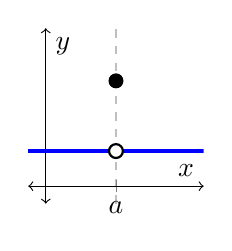
\begin{tikzpicture}[scale=1]
          \begin{axis}[
        %    axis y line = left,
        %    axis x line = bottom,
            xlabel={$x$},
            xtick       = {2},
            xticklabels = {$a$},
            ytick       = {0},
            yticklabels = {},
            samples     = 160,
            domain      = -1:5,
            restrict y to domain=-1:5,
            xmin = -0.5, xmax = 4.5,
            ymin = -0.5, ymax = 4.5,
            grid=both, grid style=dashed,
            width=1.5in, height=1.5in
          ]
          % pieces 1 and 2
          \addplot[domain=-1:5, blue, ultra thick, mark=none] {1};
          \filldraw[white] (2,1) circle (2.5pt);
          \draw[thick] (2,1) circle (2.5pt);
          \filldraw[black] (2,3) circle (2.5pt);
        \end{axis}
        \end{tikzpicture}
        %
        \hfill
        %
        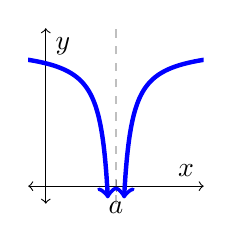
\begin{tikzpicture}[scale=1]
          \begin{axis}[
        %    axis y line = left,
        %    axis x line = bottom,
            xlabel={$x$},
            xtick       = {2},
            xticklabels = {$a$},
            ytick       = {0},
            yticklabels = {},
            samples     = 160,
            domain      = -1:5,
            restrict y to domain=-1:5,
            xmin = -0.5, xmax = 4.5,
            ymin = -0.5, ymax = 4.5,
            grid=both, grid style=dashed,
            width=1.5in, height=1.5in
          ]
          % pieces 1 and 2
          \addplot[domain=-1:1.77, blue, ultra thick, mark=none, <->] {4-abs(x-2)/(x-2)^2};
           \addplot[domain=2.23:5, blue, ultra thick, mark=none, <->] {4-abs(x-2)/(x-2)^2};
        \end{axis}
        \end{tikzpicture}
        %
        \hfill
        %
        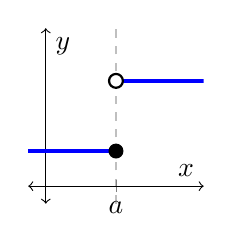
\begin{tikzpicture}[scale=1]
          \begin{axis}[
        %    axis y line = left,
        %    axis x line = bottom,
            xlabel={$x$},
            xtick       = {2},
            xticklabels = {$a$},
            ytick       = {0},
            yticklabels = {},
            samples     = 160,
            domain      = -1:5,
            restrict y to domain=-1:5,
            xmin = -0.5, xmax = 4.5,
            ymin = -0.5, ymax = 4.5,
            grid=both, grid style=dashed,
            width=1.5in, height=1.5in
          ]
          % pieces 1 and 2
          \addplot[domain=-1:2, blue, ultra thick, mark=none] {1};
          \filldraw[black] (2,1) circle (2.5pt);
          \addplot[domain=2:5, blue, ultra thick, mark=none] {3};
          \filldraw[white] (2,3) circle (2.5pt);
          \draw[thick] (2,3) circle (2.5pt);
        \end{axis}
        \end{tikzpicture}
        %
        \hfill
        %
        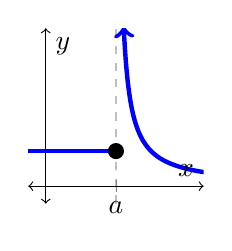
\begin{tikzpicture}[scale=1]
          \begin{axis}[
        %    axis y line = left,
        %    axis x line = bottom,
            xlabel={$x$},
            xtick       = {2},
            xticklabels = {$a$},
            ytick       = {0},
            yticklabels = {},
            samples     = 160,
            domain      = -1:5,
            restrict y to domain=-1:5,
            xmin = -0.5, xmax = 4.5,
            ymin = -0.5, ymax = 4.5,
            grid=both, grid style=dashed,
            width=1.5in, height=1.5in
          ]
          % pieces 1 and 2
          \addplot[domain=-1:2, blue, ultra thick, mark=none] {1};
          \filldraw[black] (2,1) circle (2.5pt);
          \draw[thick] (2,1) circle (2.5pt);
          \addplot[domain=2.22:5, blue, ultra thick, mark=none, <->] {1/(x-2)};
        \end{axis}
        \end{tikzpicture}
        %
        \hfill
        %
        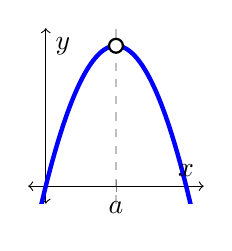
\begin{tikzpicture}[scale=1]
          \begin{axis}[
        %    axis y line = left,
        %    axis x line = bottom,
            xlabel={$x$},
            xtick       = {2},
            xticklabels = {$a$},
            ytick       = {0},
            yticklabels = {},
            samples     = 160,
            domain      = -1:5,
            restrict y to domain=-1:5,
            xmin = -0.5, xmax = 4.5,
            ymin = -0.5, ymax = 4.5,
            grid=both, grid style=dashed,
            width=1.5in, height=1.5in
          ]
          % pieces 1 and 2
          \addplot[domain=-1:5, blue, ultra thick, mark=none] {4-(x-2)^2};
          \filldraw[white] (2,4) circle (2.5pt);
          \draw[thick] (2,4) circle (2.5pt);
        \end{axis}
        \end{tikzpicture}
        %
        \hfill
        %
        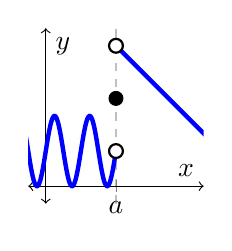
\begin{tikzpicture}[scale=1]
          \begin{axis}[
        %    axis y line = left,
        %    axis x line = bottom,
            xlabel={$x$},
            xtick       = {2},
            xticklabels = {$a$},
            ytick       = {0},
            yticklabels = {},
            samples     = 160,
            domain      = -1:5,
            restrict y to domain=-1:5,
            xmin = -0.5, xmax = 4.5,
            ymin = -0.5, ymax = 4.5,
            grid=both, grid style=dashed,
            width=1.5in, height=1.5in
          ]
          % pieces 1 and 2
          \addplot[domain=-1:2, blue, ultra thick, mark=none] {1+sin(deg(x)*3.141*2)};
          \filldraw[white] (2,1) circle (2.5pt);
          \draw[thick] (2,1) circle (2.5pt);
          \addplot[domain=2:5, blue, ultra thick, mark=none] {6-x};
          \filldraw[white] (2,4) circle (2.5pt);
          \draw[thick] (2,4) circle (2.5pt);
          \filldraw (2,2.5) circle (2.5pt);
        \end{axis}
        \end{tikzpicture}
    \hfill\,\\


%
\begin{enumerate}
\item[i.] For each graph above, label the graph as depicting a removable, jump, or infinite discontinuity by writing the letters ``RD", ``JD", or ``ID" (respectively).\\
\item[ii.] If a function is discontinuous at a number, then the function must violate at least one of the three conditions. For each graph above, label the graph with the number(s) of the continuity condition(s) the graph violates in the space below the graph.\\
\item[iii.] Based on your labeling, characterize each type of discontinuity by which continuity conditions must be violated.
\end{enumerate}
    
%%%%%%%%%%%%%%%%%%%%%%%%%%%%%%%%%%%%%%%%%%%%%%%%%%%%%
%%%%%%%%%%% END PROBLEM L1 %%%%%%%%%%%%%%%%%%%%%%%%%%
%%%%%%%%%%%%%%%%%%%%%%%%%%%%%%%%%%%%%%%%%%%%%%%%%%%%%

\newpage

%%%%%%%%%%%%%%%%%%%%%%%%%%%%%%%%%%%%%%%%%%%%%%%%%%%%%
%%%%%%%%%%% BEGIN PROBLEM P1 %%%%%%%%%%%%%%%%%%%%%%%%
%%%%%%%%%%%%%%%%%%%%%%%%%%%%%%%%%%%%%%%%%%%%%%%%%%%%%

\item In the game \textit{Dungeons \& Dragons}, damage is frequently determined by rolling dice. The notation ``$N$d$X$'' means rolling $N$ dice that each have $X$ faces (numbered $1$ to $X$). We assume every face on a die has an equal probability of occurring. We will also ignore some of the aspects of the game for simplicity of the problem.

You have two options for your turn:
\begin{itemize}
    \item \textbf{Melee Attack:} You deal $2$ bonus damage plus the result of a 4-sided die ($2 + 1$d$4$). For example, if you roll $3$ on the dice, you deal $5$ damage total.
    \item \textbf{Frostbite:} You deal damage equal to the result of a 6-sided die ($1$d$6$).
\end{itemize}

Let $M$ be the discrete random variable for the Melee damage, and let $F$ be the discrete random variable for the Frostbite damage.

\begin{enumerate}
    \item Write down the probability mass function for the Melee attack, $p_M(m)$, and the Fire Bolt spell, $p_F(f)$. (You may use tables or piecewise functions).

    \vfill
    \vfill

    \item Calculate the probability of dealing \textbf{3 or more} damage for each method. That is, find $P(M \geq 3)$ and $P(F \geq 3)$.

    \vfill
    \vfill

    \item Which option, on average, deals more damage? \textit{Hint: compute the expected damage for each option}

    \vfill

    \vfill

\end{enumerate}

%%%%%%%%%%%%%%%%%%%%%%%%%%%%%%%%%%%%%%%%%%%%%%%%%%%%%
%%%%%%%%%%% END PROBLEM P1 %%%%%%%%%%%%%%%%%%%%%%%%%%
%%%%%%%%%%%%%%%%%%%%%%%%%%%%%%%%%%%%%%%%%%%%%%%%%%%%%

\newpage

%%%%%%%%%%%%%%%%%%%%%%%%%%%%%%%%%%%%%%%%%%%%%%%%%%%%%
%%%%%%%%%%% BEGIN PROBLEM P2 %%%%%%%%%%%%%%%%%%%%%%%%
%%%%%%%%%%%%%%%%%%%%%%%%%%%%%%%%%%%%%%%%%%%%%%%%%%%%%

\item 
\begin{enumerate}
    \item For each graph below indicate whether this could be a part of a probability density function (PDF), cumulative distribution function (CDF), both or neither. Explain your choice.
        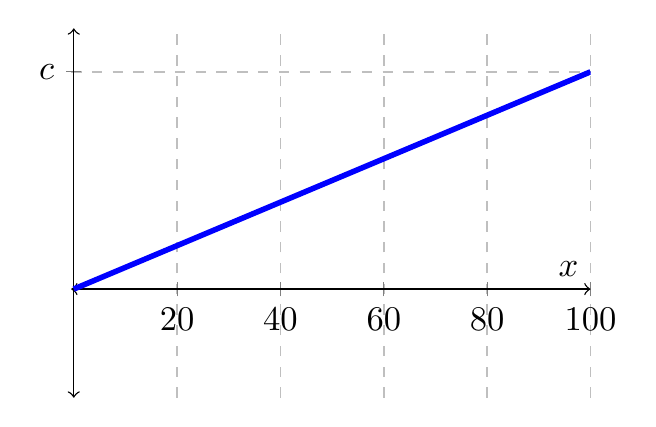
\begin{tikzpicture}[scale=1.25]
          \begin{axis}[
            xlabel={$x$},
            ylabel={\empty},
            %grid = major,
            xtick       = {0,20,40,60,80,100},
            xticklabels = {$0$,$20$,$40$,$60$,$80$,$100$},
            ytick       = {0,1},
            yticklabels = {$0$, $c$},
            samples     = 320,
            domain      = 0:101,
            restrict y to domain=-2:5,
            xmin = -0.5, xmax = 100,
            ymin = -0.5, ymax = 1.2,
            height=2.1in, width=2.7in,
            grid=both, grid style=dashed]
            %\addplot[domain=0:4, blue, ultra thick, mark=none] {4-4/2^x};
            %\addplot[domain=5:8, blue, ultra thick, mark=none] {};
            %\node at (4,3) {$r(t)$};
            \draw[ultra thick, blue,-] (0,0) -- (100, 1);
        \end{axis}
    \end{tikzpicture}
    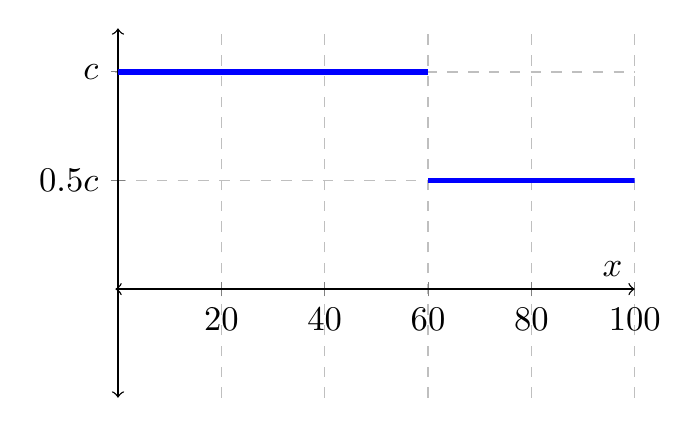
\begin{tikzpicture}[scale=1.25]
          \begin{axis}[
            xlabel={$x$},
            ylabel={\empty},
            %grid = major,
            xtick       = {0,20,40,60,80,100},
            xticklabels = {$0$,$20$,$40$,$60$,$80$,$100$},
            ytick       = {0,0.5,1},
            yticklabels = {$0$, $0.5c$, $c$},
            samples     = 320,
            domain      = 0:101,
            restrict y to domain=-2:5,
            xmin = -0.5, xmax = 100,
            ymin = -0.5, ymax = 1.2,
            height=2.1in, width=2.7in,
            grid=both, grid style=dashed]
            %\addplot[domain=0:4, blue, ultra thick, mark=none] {4-4/2^x};
            %\addplot[domain=5:8, blue, ultra thick, mark=none] {};
            %\node at (4,3) {$r(t)$};
            \draw[ultra thick, blue,-] (0,1) -- (60, 1);
            \draw[ultra thick, blue,-] (60,0.5) -- (100, 0.5);
        \end{axis}
        \end{tikzpicture}
        
        \vspace{1cm}
        
        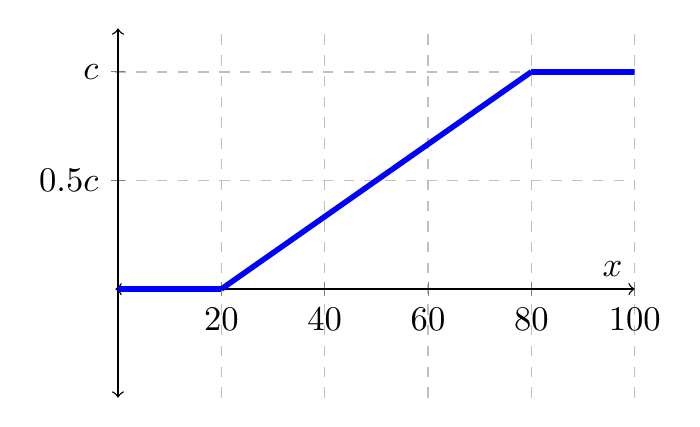
\begin{tikzpicture}[scale=1.25]
          \begin{axis}[
            xlabel={$x$},
            ylabel={\empty},
            %grid = major,
            xtick       = {0,20,40,60,80,100},
            xticklabels = {$0$,$20$,$40$,$60$,$80$,$100$},
            ytick       = {0,0.5,1},
            yticklabels = {$0$, $0.5c$, $c$},
            samples     = 320,
            domain      = 0:101,
            restrict y to domain=-2:5,
            xmin = -0.5, xmax = 100,
            ymin = -0.5, ymax = 1.2,
            height=2.1in, width=2.7in,
            grid=both, grid style=dashed]
            %\addplot[domain=0:4, blue, ultra thick, mark=none] {4-4/2^x};
            %\addplot[domain=5:8, blue, ultra thick, mark=none] {};
            %\node at (4,3) {$r(t)$};
            \draw[ultra thick, blue,-] (0,0) -- (20, 0);
            \draw[ultra thick, blue,-] (20,0) -- (80, 1);
            \draw[ultra thick, blue,-] (80,1) -- (100, 1);
        \end{axis}
        \end{tikzpicture}
                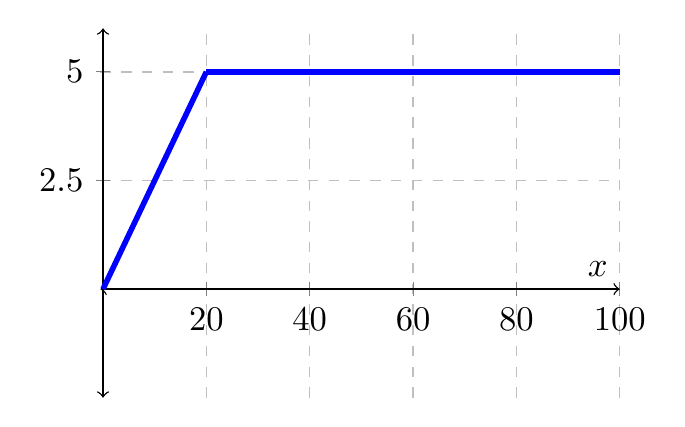
\begin{tikzpicture}[scale=1.25]
          \begin{axis}[
            xlabel={$x$},
            ylabel={\empty},
            %grid = major,
            xtick       = {0,20,40,60,80,100},
            xticklabels = {$0$,$20$,$40$,$60$,$80$,$100$},
            ytick       = {0,0.5,1},
            yticklabels = {$0$, $2.5$, $5$},
            samples     = 320,
            domain      = 0:101,
            restrict y to domain=-2:5,
            xmin = -0.5, xmax = 100,
            ymin = -0.5, ymax = 1.2,
            height=2.1in, width=2.7in,
            grid=both, grid style=dashed]
            %\addplot[domain=0:4, blue, ultra thick, mark=none] {4-4/2^x};
            %\addplot[domain=5:8, blue, ultra thick, mark=none] {};
            %\node at (4,3) {$r(t)$};
            \draw[ultra thick, blue,-] (0,0) -- (20, 1);
            \draw[ultra thick, blue,-] (20,1) -- (80, 1);
            \draw[ultra thick, blue,-] (80,1) -- (100, 1);
        \end{axis}
        \end{tikzpicture}
    \vspace{1cm}
    \item For each picture above that can be a PDF, find the corresponding CDF. For each picture above that can be a CDF, find the corresponding PDF. 
    \vfill
\end{enumerate}
\end{enumerate}

%%%%%%%%%%%%%%%%%%%%%%%%%%%%%%%%%%%%%%%%%%%%%%%%%%%%%
%%%%%%%%%%% END PROBLEM P2 %%%%%%%%%%%%%%%%%%%%%%%%%%
%%%%%%%%%%%%%%%%%%%%%%%%%%%%%%%%%%%%%%%%%%%%%%%%%%%%%


\end{document}